\chapter{Evaluación de impactos}\label{cap:6}
\lettrine{F}{recuentemente, en especial en ingeniería}, los proyectos tienen la obligación de identificar y realizar un estudio detallado de los impactos medioambientales, sociales y económicos derivados. Además, también es habitual hacer ---antes de la identificación de impactos--- un análisis de los distintos grupos de interés (\emph{stakeholders}) involucrados directa o indirectamente en el portafolio en cuestión. En la actualidad, adicionalmente, un grupo cada vez mayor de las empresas que constituyen el tejido empresarial internacional están comprometidas y trabajan siguiendo uno o varios de los \acrfull{ods}, adoptados por la \acrfull{onu} en $2015$, para conseguir los $17$ objetivos aprobados por los Estados miembros en la Agenda $2030$. Este capítulo \S\ref{cap:6}, aunque brevemente, presenta los principales impactos y grupos de interés relacionados con este trabajo, esquematizados en la Figura \ref{fig:6.1}.

Para comenzar, los principales impactos medioambientales asociados a este proyecto están limitados a la fabricación y consumo eléctrico de los equipos informáticos utilizados, principalmente los ordenadores personales y servidores remotos empleados. Un análisis más extenso de los equipos electrónicos, debería contemplar el ciclo de vida completo, desde la obtención de las materias primas, pasando por el transporte, hasta la fabricación. El consumo energético está centrado fundamentalmente en el servidor remoto, encargado de ejecutar las simulaciones, mientras que el ordenador personal ha realizado tareas de menor coste computacional. En este aspecto, una mayor profundidad de estudio necesitaría desglosar, por ejemplo, las distintas fuentes de energía que han alimentado los sistemas informáticos.

Por otro lado, teniendo en cuenta los avances actuales en esta línea de investigación, los láseres de rayos X blandos \acrshort{sxrl} basados en plasmas densos, aunque prometedores, es muy difícil predecir cuáles pudieran ser las repercusiones sociales de desarrollar completamente, por ejemplo a nivel industrial, estos sistemas láser. En el futuro, sustituir instalaciones complejas y de gran tamaño, como láseres de electrones libres (\acrshort{fel}), permitiría reducir el coste de inversión (entre \$$100$M y \$$1000$M), mantenimiento (\$$100$M) y desmantelamiento, intercambiándolas por estos láseres. En este sentido, el impacto económico está destinado a disminuir inversiones de estas magnitudes, mientras que el impacto social estaría vinculado a campos de investigación como la biología molecular, o en medicina y cirugía.

Volviendo a los grupos de interés, establecer cuáles son los agentes más importantes interesados en esta línea de investigación es básico para conocer si los objetivos establecidos dan respuesta a sus necesidades y, en definitiva, si es relevante. Los grupos de interés existentes pueden distinguirse como dos tipos separados: directos e indirectos.

\begin{itemize}

    \item Directos. Los agentes individuales directamente involucrados son: el estudiante, autor del trabajo, y el profesor tutor, el Dr. Eduardo Oliva, encargado de dirigir el proyecto. Los resultados obtenidos han permitido continuar trabajos anteriores en materia de láseres \acrshort{sxrl} basados en plasmas de \ce{Kr^{8+}}, mejorando la comprensión de aspectos relacionados con la amplificación obtenida. A mayor distancia, aunque importantes, están el Instituto de Fusión Nuclear \enquote{Guillermo Velarde} (IFN-GV) donde está asentado el profesor tutor, perteneciente al Departamento de Ingeniería Energética (DIE) de la Escuela Técnica Superior de Ingenieros Industriales (ETSII) en la Universidad Politécnica de Madrid (UPM), última receptora de los resultados presentados a través de la memoria del trabajo.
    \item Indirectos. A nivel nacional, aunque no este proyecto en particular, el ahora Ministerio de Ciencia, Innovación y Universidades ha financiado varios trabajos y grupos de investigación en esta área, mientras que a nivel internacional, la Unión Europea también ha participado activamente otorgando financiación en este ámbito. Fuera del territorio nacional también se encuentra el \emph{\acrfull{loa}}, en Francia, donde los experimentos fueron llevados a cabo, proporcionando los medios materiales y humanos necesarios para su ejecución.

\end{itemize}

Por último, en cuanto a la Agenda $2030$, la introducción y promoción de nuevas tecnologías como las estudiadas durante este trabajo están enmarcadas dentro del objetivo $9$, \enquote{Industria, Innovación e Infraestructura}, especialmente la inversión en tecnologías avanzadas y la mejora de las capacidades tecnológicas en industria e investigación. En cierto modo, estas actividades pueden favorecer un uso más eficientes de los recursos, a la vez que generan nuevos empleos e ingresos. Además, en el futuro, como se ha mencionado anteriormente, las posibles aplicaciones tecnológicas en biología y medicina también ayudarían a mejorar, de acuerdo con el objetivo $3$ \enquote{Salud y Bienestar}, la calidad de vida de las personas, por ejemplo, en epidemias o pandemias que necesiten estudiar la estructura de bacterias o virus.

\begin{figure}[htbp]
  \centering
  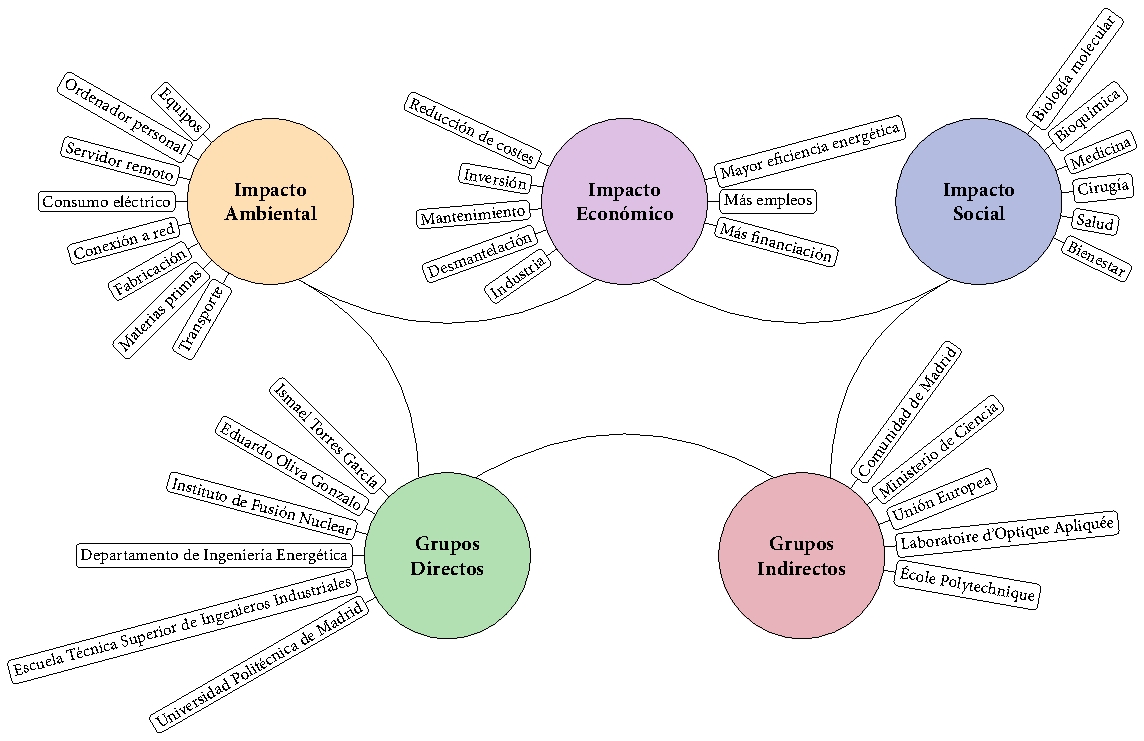
\includegraphics[width=\textwidth]{Figuras/ch6_impcts.pdf}
  \caption{Mapa de impactos y grupos de interés participantes.}
  \label{fig:6.1}
\end{figure}
